\documentclass[11pt,a4paper]{article}
\usepackage{caption}
\usepackage[utf8]{inputenc}
\usepackage{supertabular}
\usepackage[T1]{fontenc}
\usepackage{icomma}
\usepackage{array} 
\usepackage{color}
\usepackage{amsmath,mathtools}
\usepackage{bbm}
\usepackage{amssymb,amsfonts}
\usepackage{esint}
\usepackage[table,xcdraw,dvipsnames]{xcolor}
\usepackage{listings}
\lstset{basicstyle=\ttfamily,
  showstringspaces=false,
  commentstyle=\color{red},
  keywordstyle=\color{blue}
}
\usepackage{fancyvrb}
\usepackage{verbatim}
\DefineVerbatimEnvironment%
      {verbatimprog}%
      {Verbatim}%
      {fontsize=\footnotesize}%
\usepackage{multirow}
\usepackage{graphicx}
\usepackage{subcaption}
\usepackage{filecontents}
\usepackage{float}
\usepackage{tikz}
\usepackage[left=2.5cm,right=2.5cm,top=3cm,bottom=3cm]{geometry}
\usepackage{hyperref}
\usepackage[english]{babel}
\usepackage[bottom]{footmisc}
\usepackage{gensymb}
\usepackage{tabulary}
\usepackage{fancyhdr}
\usepackage{siunitx}
\usepackage{textcomp}
\usepackage{endnotes}
\usepackage[siunitx]{circuitikz}
\newcommand{\HRule}{\rule{\linewidth}{0.5mm}}
\usepackage{parskip}
\setlength{\parindent}{0cm}
\setlength{\parskip}{15pt}
\setlength\extrarowheight{2pt}
\usepackage{tcolorbox}
\usepackage{multirow}
\usepackage{enumitem}
\usepackage[ampersand]{easylist}
%\usepackage{subfigure}
\usepackage{hhline}
\usepackage{datetime}
\usepackage{float}
\usepackage{tikz}
\usetikzlibrary{matrix,chains,positioning,decorations.pathreplacing,arrows}
\usepackage{fancyhdr}
\usepackage{lastpage}
\lstset{
  literate=
  {á}{{\'a}}1 {é}{{\'e}}1 {í}{{\'i}}1 {ó}{{\'o}}1 {ú}{{\'u}}1
  {Á}{{\'A}}1 {É}{{\'E}}1 {Í}{{\'I}}1 {Ó}{{\'O}}1 {Ú}{{\'U}}1
  {à}{{\`a}}1 {è}{{\`e}}1 {ì}{{\`i}}1 {ò}{{\`o}}1 {ù}{{\`u}}1
  {À}{{\`A}}1 {È}{{\'E}}1 {Ì}{{\`I}}1 {Ò}{{\`O}}1 {Ù}{{\`U}}1
  {ä}{{\"a}}1 {ë}{{\"e}}1 {ï}{{\"i}}1 {ö}{{\"o}}1 {ü}{{\"u}}1
  {Ä}{{\"A}}1 {Ë}{{\"E}}1 {Ï}{{\"I}}1 {Ö}{{\"O}}1 {Ü}{{\"U}}1
  {â}{{\^a}}1 {ê}{{\^e}}1 {î}{{\^i}}1 {ô}{{\^o}}1 {û}{{\^u}}1
  {Â}{{\^A}}1 {Ê}{{\^E}}1 {Î}{{\^I}}1 {Ô}{{\^O}}1 {Û}{{\^U}}1
  {œ}{{\oe}}1 {Œ}{{\OE}}1 {æ}{{\ae}}1 {Æ}{{\AE}}1 {ß}{{\ss}}1
  {ű}{{\H{u}}}1 {Ű}{{\H{U}}}1 {ő}{{\H{o}}}1 {Ő}{{\H{O}}}1
  {ç}{{\c c}}1 {Ç}{{\c C}}1 {ø}{{\o}}1 {å}{{\r a}}1 {Å}{{\r A}}1
  {€}{{\EUR}}1 {£}{{\pounds}}1
}
\usepackage{emptypage}
%\renewcommand\headrulewidth{1pt}
%\fancyhead[L]{\textbf{Titre}}
%\fancyhead[C]{}
\def \kawFigPath {Output/Images}
\newcommand{\terminal}[1]{
    \begin{tcolorbox}[boxrule=0.25mm,left=0mm,right=0mm]
    \footnotesize{\texttt{#1}}
    \end{tcolorbox}}
\newcommand\commit[2]{\node[commit] (#1) {}; \node[clabel] at (#1) {\texttt{#1}: #2};}
\newcommand\ghost[1]{\coordinate (#1);}
\newcommand\connect[2]{\path (#1) to[out=90,in=-90] (#2);}
%\fancyhead[R]{Prénom Nom}
%\renewcommand\footrulewidth{1pt}
%\fancyfoot[C]{\textbf{Page \thepage/\pageref{LastPage}}}
%\fancyfoot[R]{\today \quad \currenttime }
\begin{document}

\begin{titlepage}
\begin{center}

\includegraphics[scale=0.3]{\kawFigPath /IMTA.jpg}
\line(1,0){400}\\
[2mm]
\begin{large}
\textbf{Machine Learning - Binary Classification}\\ 
\end{large}
\line(1,0){250}\\
[1.5cm]
by\\
QUINTANA Gonzalo\\
MARRA Tales\\
WANG Lei\\
AGUDELO Santiago\\
[2.5cm]
UE A - Introduction to Machine Learning\\
[2.5cm]
Supervisor:\\
Professor Elza DUPRAZ\\
[4cm]
TAF Mathematical Computing Engenieering\\
IMT Atlantique\\
[1cm]
\today
\end{center} 
\end{titlepage}

\section*{Introduction}

The following report summarizes our work on Machine Learning course project. This project consisted in binary classification of two datasets. The first dataset we took into account was the “Banknote Authentication Dataset”, in which data was extracted from images that were taken for evaluating the authentication procedure for banknotes. The second dataset we considered was the “Chronic Kidney disease Dataset”, which consisted in 25 features which may allow predicting a patient with chronic kidney disease.

The main goal of the project was to apply on practical datasets some of the different machine learning algorithms that were introduced during course sessions, all this by adopting a teamwork-based collaborative approach. It was also searched to raise consciousness about good programming practices, which are necessary for all developed codes to be organized, understandable and properly documented. 

First, the datasets will be described as well as the pre-processing they require. Then, the binary classification problem will be solved for both datasets by using machine learning algorithms such as support vector machines, neural networks, decision trees and clustering techniques. The obtained results will be presented and discussed; this will allow evaluating the pertinence of the different algorithms in terms of their performance and complexity. In the end, a conclusion section will summarize the main points of discussion as well as the principal difficulties we encountered during the project’s realization. 

\section{Datasets: description and pre-processing}

\subsection{Banknote Authentication Dataset}
These data were extracted from images that were taken from genuine and forged banknote-like specimens. These images have a size of 400x400 pixels with a resolution of about 660 dpi. In addition, wavelet transform was used to extract different features from images.

The variance, skewness and curtosis of the wavelet transformed image, the entropy of the image and its class are included in the dataset. This last information sets whether the image corresponds to a genuine of a forged specimen; it is therefore our objective to develop machine learning algorithms allowing to predict the image's class from information on the dataset. 

\subsection{Chronic Kidney Disease Dataset}
The data was taken over a 2 months period in India. It includes 25 features that allow predicting the presence of chronic kidney disease. Our goal is therefore to use the information contained in the dataset to determine through machine learning algorithms whether a patient suffers from this disease (we will call this case ckd) or not (we will call this case notckd). 

\subsection{Preprocessing}

The datasets we worked on encountered problems such as missing values, out-of-range values, invalid characters, non-centered data, etc. Also, some of the data corresponded to text that cannot be directly processed; therefore, a conversion to a numerical format is necessary.

For pre-processing data, we developed a module that can be applied to a general dataset.This way, we could use the same procedure to pre-process both of the datasets concerned by this project. 
In such module, the user must indicate the repertory where data are localized and whether the header arrow and the index column are present or not. The user is also requested if text data should be transformed into numerical data. 

The following steps allow obtaining a exploitable dataset: 
\begin{enumerate}
    \item The files (.text or .csv) are read through pandas in Python. 
    \item Features and targets are separated. 
    \item For each feature and target, the strings they contain are identified. In this same step, all special characters are left behind. 
    \item Data are cleansed. If there happens to be a missing value in a numerical column (feature), it is replaced by the average value of the column. For modal columns (i.e, the columns that contain strings), strings are converted into a numerical format. For example, the words yes/no are converted to a binary format 1/0. If these columns happen to have missing values, they are filled with random data in a way the proportion of the values in the column doesn't change. 
    \item Features are normalized (the mean is subtracted and the result is scaled in order to have unit variance). 
    
\end{enumerate}
In all the algorithms that will be further mentioned, the proportion of the training set and the test set is of 2/3 and 1/3 of the dataset, respectively. 

\section{PCA}
 When representing each exemplary as a point in the variables space, principal components are obtained as the succession of orthogonal vectors that best fits the data (this is, the succession of vectors that minimizes the error one commits when projecting the data into these vectors). It is possible to calculate such vectors as the eigenvectors of the correlation matrix of data; each of which is associated to an eigenvalue that indicates the total contribution of each principal component to the variation of the data. 

When taking into account the most important components (this is, those corresponding to the highest eigenvalues), it is possible to reduce the problem to a lower dimension. 

Figure \ref{PCA1} shows the correlation circle of features in the banknote dataset. When representing features as vectors in the individual space, the circle is obtained by projecting the features in the two dimensional space generated by the two components corresponding to the highest eigenvalues. This circle allows to determine the correlation behavior between the variables themselves and between variables and principal components. 
The percentages on the plot represent the amount of variation of the model that the principal components stand for. 
It can be seen that skewness and curtosis are well explained by the component PC1 since the angle they form with this component is small. The directions of the vectors show that skewness is positive correlated with PC1 while curtosis is negatively correlated to this component. Entropy and variance are more correlated to PC2 than they are to PC1, and the existing correlation is positive since they point in the direction of PC2. Also, the length of the vectors in the graph tells us how close the actual features are to the the plane generated by the two principal components. The longer the length, the closest the features are to the plane generated by PC1 and PC2 and, in consequence, the more trustful the representation of data in terms of these components is. 

It is important to recall that representation using PC1 and PC2 stands for 86.7\% of variation of the model. There is a part of the variation that isn't explained by these components and therefore, if data were reduced to just these two dimensions for further classification, the results thrown by different classifiers might not fit well enough the original data. Indeed, in table \ref{tablePCA1} (presented at the end of the document) a comparison is made between different classifiers when using these PCA components and when using all available data. It can be seen that the overall performance is lowered when only considering PCA components, which is explained by the fact that the PCA components don't stand for all variation in the data. 

Concerning the kidney disease database, binary variables were not taken into account for PCA analysis. We calculated the principal components of the quantitative variables and we used the first K principal components plus the binary features to perform classification of data, first with K=2 and then with K=7. Results are presented at table \ref{tablePCA2} (in the end of the document). It can be stated that lowering the dimension of the quantitative data leads to a similar (and in some cases, even better) classification performance in terms of different metrics. In the original dataset, some of the features may not be related with the disease and considering them in classification introduces a certain nuisance that lowers the classifier's performance. Also, in addition of the quantitative features used in PCA calculation, binary features were  considered in the classification process. Hence, the influence of binary variables is always present, which means the number of components actually taken into account was never as low as 2. 

\begin{figure}[ht]
    \centering
    \begin{subfigure}[b]{0.45\textwidth} % "0.45" donne ici la largeur de l'image
        \centering 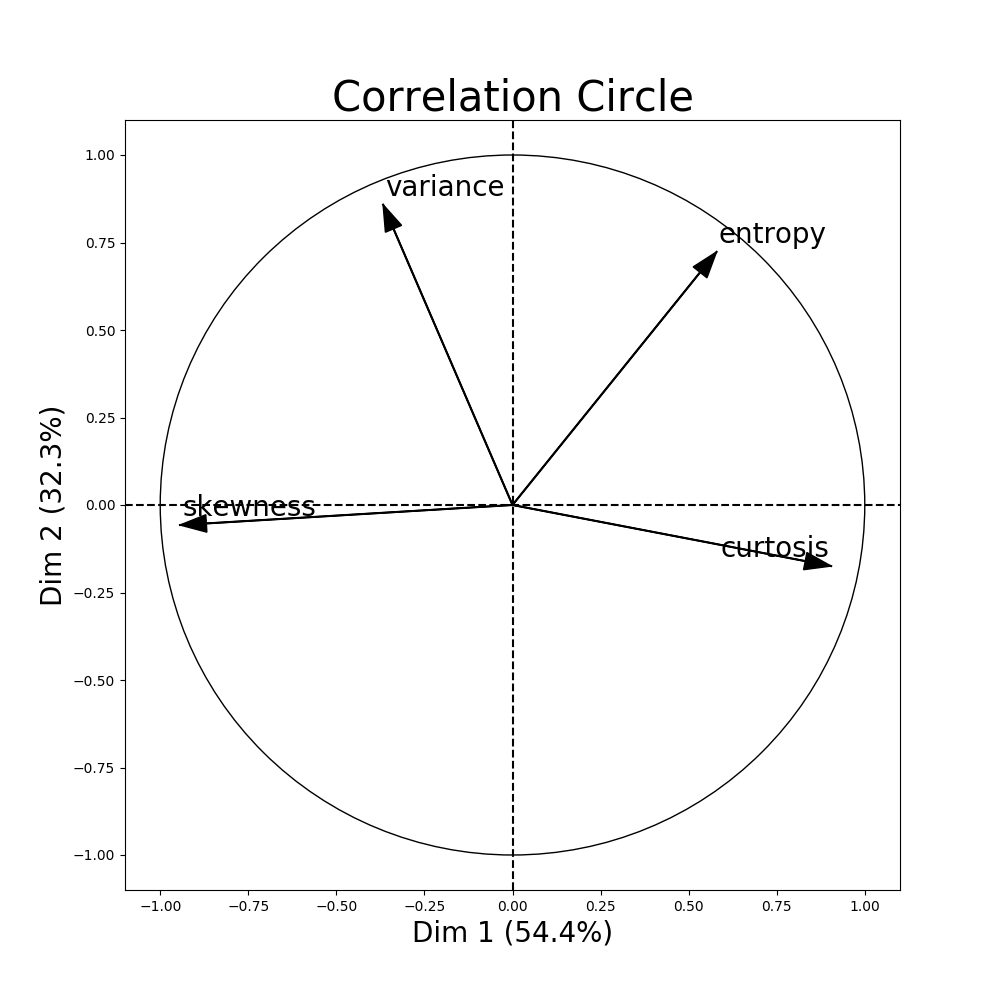
\includegraphics[width=\textwidth]{\kawFigPath /PCA_for_dataset_bank-note.png}
        \caption{Bank note dataset}\label{ligne_on}
    \end{subfigure}
    ~
    \begin{subfigure}[b]{0.45\textwidth}
        \centering 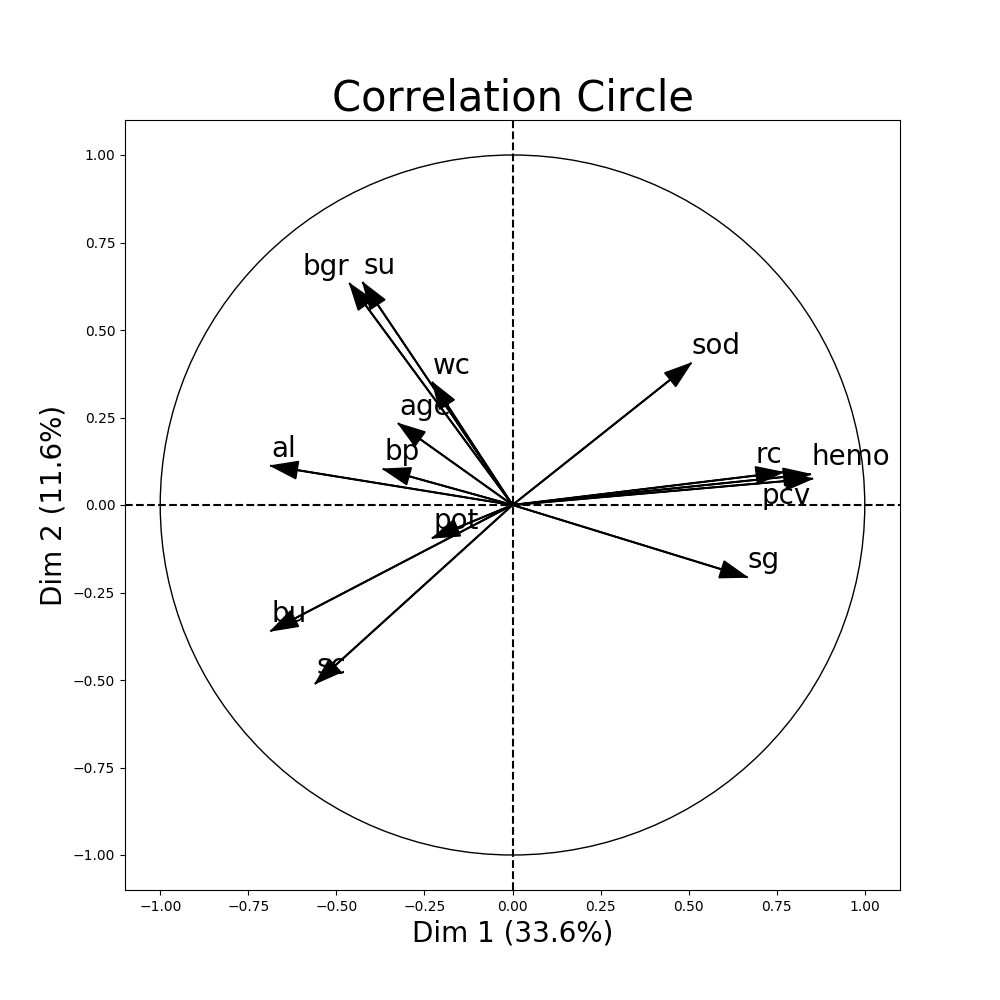
\includegraphics[width=\textwidth]{\kawFigPath /PCA_for_dataset_kidney-disease.png}
        \caption{Kidney disease dataset}\label{ligne_off}
    \end{subfigure}
    \caption{Correlation Circles obtained through PCA for the two datasets}\label{PCA1}

\end{figure}

\section{SVM}
The main goal of this algorithm is to separate binary data through an hyperplane. Since data may not be linearly separable, the kernel trick may be used to map data into a higher dimensional space, in which it would become linearly separable. SVM was implemented through scikit-learn library. This function solves the following optimization problem, given training vectors $x_i$ and $y_i \in \lbrace0,1\rbrace$ : 
   $$ \min\limits_{w, \zeta} \hspace{0.5cm} \frac{1}{2} w^Tw + C\sum_{i=1}^{n} \zeta_i$$
$$st \hspace{0.5cm} y_i(w^T\varphi(x_i)+b \geq 1- \zeta_i$$ 
   $$\zeta_i \geq 0$$
Its dual problem: 
   $$ \min\limits_{\alpha} \hspace{0.5cm} \frac{1}{2} \alpha^TQ\alpha -e^T\alpha$$
$$st \hspace{0.5cm} y^T\alpha=0$$ 
   $$0 \leq \alpha_i \leq C$$

$e$ is an only ones vector and the matrix $Q$ is defined as $Q_{ij}=y_iy_jK(x_i,x_j)$, where $K(x_i,x_j)=\varphi(x_i)^T\varphi(x_j)$ is the kernel that implicitly maps our data into a higher dimensional space. 

For our implementation, we defined $K(x,x')=exp(-\gamma ||x-x'||^2)$ with $\gamma=\frac{1}{N\cdot var(x)}$. 
The following figures show the confusion matrices for training and test data that were obtained when running the algorithm on both datasets. It can be stated that this algorithm reaches a perfect performance when applied on the banknote dataset : indeed, none of the fake bills in the test set is labeled as true and vice-versa. When looking at the kidney disease dataset, none of the healthy patients from the test data are labeled as sick, but as much as 1\% of the sick ones are diagnosed as healthy. 

\begin{figure}[H]
    \centering
    \begin{subfigure}[b]{0.45\textwidth} % "0.45" donne ici la largeur de l'image
        \centering 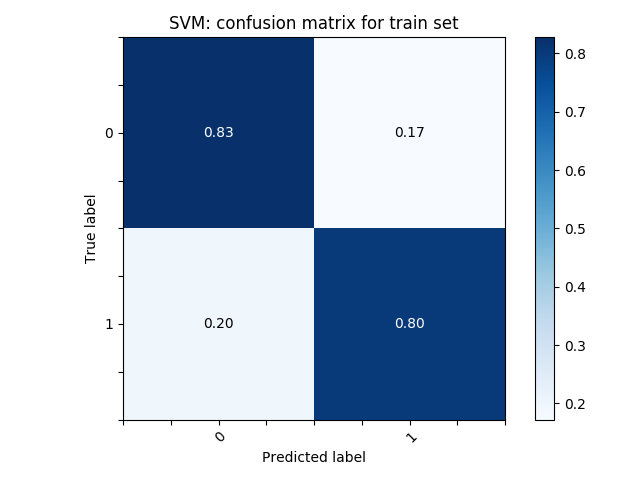
\includegraphics[width=\textwidth]{\kawFigPath /SVM-bank-note-cm-train.png}
        \caption{Confusion matrix of training data}\label{ligne_on}
    \end{subfigure}
    ~
    \begin{subfigure}[b]{0.45\textwidth}
        \centering 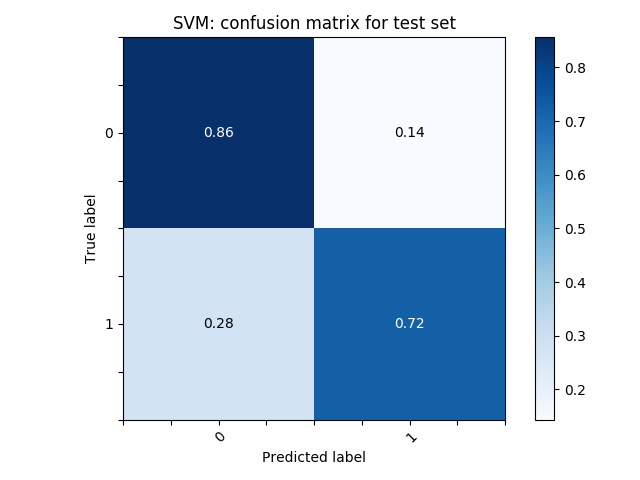
\includegraphics[width=\textwidth]{\kawFigPath /SVM-bank-note-cm-test.png}
        \caption{Confusion matrix test data}\label{ligne_off}
    \end{subfigure}
    \caption{Confusion matrices in the Banknote dataset}\label{figxx}
\end{figure}

\begin{figure}[H]
    \centering
    \begin{subfigure}[b]{0.45\textwidth} % "0.45" donne ici la largeur de l'image
        \centering 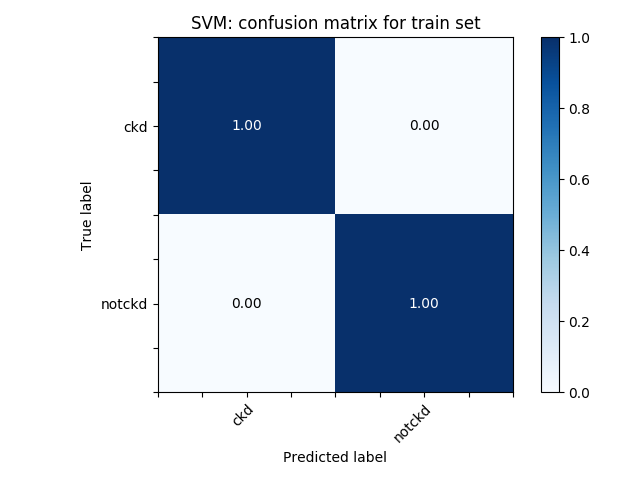
\includegraphics[width=\textwidth]{\kawFigPath /SVM-kidney-disease-cm-train.png}
        \caption{Confusion matrix of training data}\label{ligne_on}
    \end{subfigure}
    ~
    \begin{subfigure}[b]{0.45\textwidth}
        \centering 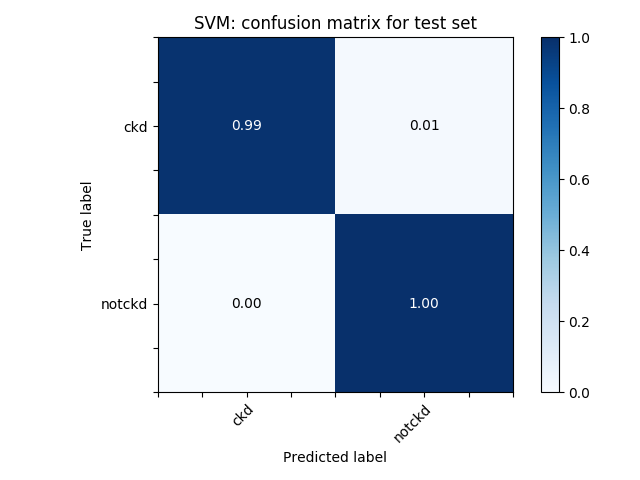
\includegraphics[width=\textwidth]{\kawFigPath /SVM-kidney-disease-cm-test.png}
        \caption{Confusion matrix test data}\label{ligne_off}
    \end{subfigure}
    \caption{Confusion matrices in the Kidney Disease dataset}\label{figxx}
\end{figure}

\section{KNN}
KNN is a non-parametric method used for classification. This algorithm requires placing a certain number of trained examples in the feature space (the class of these examples is therefore known in advance). A new sample is introduced and is classified in function of the class of its K nearest neighbors, where K is a parameter one must previously fix and neighborhood is defined in function a metric that is usually the euclidean distance. The class that will be assigned to the new sample is generally the most frequent one among its K closest neighbors. 
From a statistical approach, it can be shown that this classification rule is actually the one that maximizes the posterior probability $p(y|x)$, where $y$ stands for the class and $x$ for the sample to be classified. 

The following figures show the confusion matrices when applying this algorithm to both datasets. It can be seen that KNN has an outstanding performance on the test data corresponding to the banknote dataset. Indeed, none of the examples are misclassified. When applying the algorithm to the Kidney Dataset, however, it can be seen that even though no healthy patient is diagnosed as sick, as much as 6\% of the sick ones are diagnosed as healthy, which is considerably high and results in a bad performance of KNN for this specific application. 

\begin{figure}[ht]
    \centering
    \begin{subfigure}[b]{0.45\textwidth} % "0.45" donne ici la largeur de l'image
        \centering 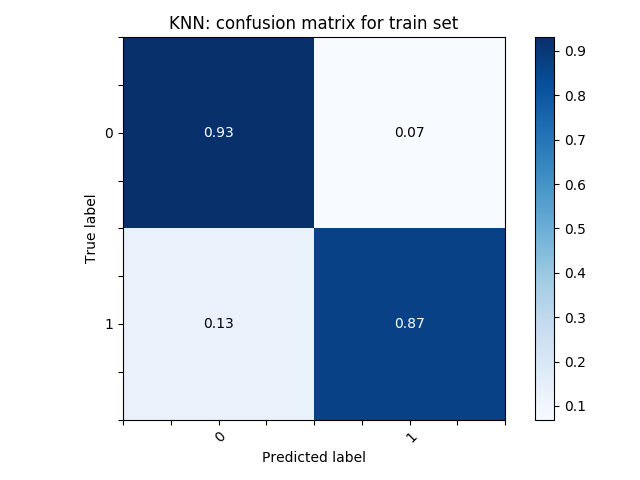
\includegraphics[width=\textwidth]{\kawFigPath /KNN-bank-note-cm-train.png}
        \caption{Confusion matrix of training data}\label{ligne_on}
    \end{subfigure}
    ~
    \begin{subfigure}[b]{0.45\textwidth}
        \centering 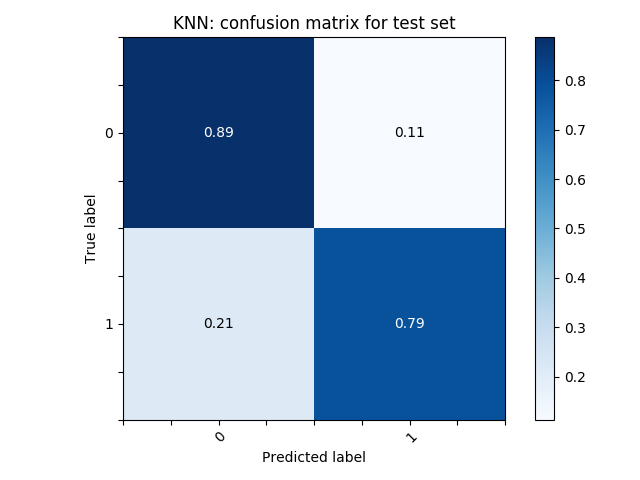
\includegraphics[width=\textwidth]{\kawFigPath /KNN-bank-note-cm-test.png}
        \caption{Confusion matrix test data}\label{ligne_off}
    \end{subfigure}
    \caption{Confusion matrices in the Banknote dataset}\label{figxx}
\end{figure}

\begin{figure}[ht]
    \centering
    \begin{subfigure}[b]{0.45\textwidth} % "0.45" donne ici la largeur de l'image
        \centering 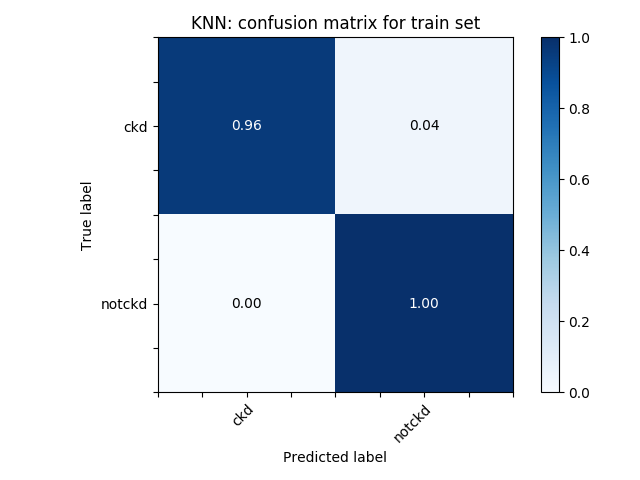
\includegraphics[width=\textwidth]{\kawFigPath /KNN-kidney-disease-cm-train.png}
        \caption{Confusion matrix of training data}\label{ligne_on}
    \end{subfigure}
    ~
    \begin{subfigure}[b]{0.45\textwidth}
        \centering 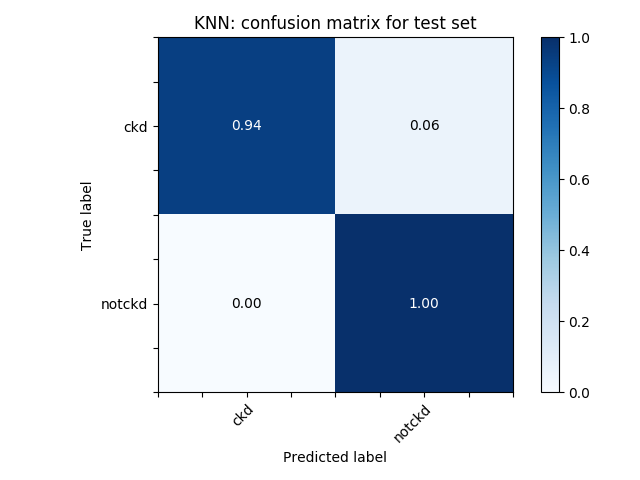
\includegraphics[width=\textwidth]{\kawFigPath /KNN-kidney-disease-cm-test.png}
        \caption{Confusion matrix test data}\label{ligne_off}
    \end{subfigure}
    \caption{Confusion matrices in the Kidney Disease dataset}\label{figxx}
\end{figure}

\section{Neural networks}
A four layer neural network was implemented by using the library Keras. Each neuron's output is a function of the weighted sum of its inputs. Such function is known as activation function and it determines whether and in what extent the neuron's output is propagated through the network and affect the overall system's output. 

The first layer uses five neurons with a ReLU activation function; the second layer consists in three neurons with a tanh activation function; the third layer is composed of two neurons with same activation function as the former, and the final layer consists of a single neuron with a sigmoid activation function. 

The neural network approach leads to the confusion matrices shown below. For the banknote dataset, 1\% of the fake bills are labeled as real and vice-versa. Concerning the kidney disease set, as much as 2\% of the healthy patients as diagnosed as sick and as much as 1\% of the sick ones are diagnosed as healthy. SVM performs better than this neural network in the first dataset, while it has a similar performance when applied on the second dataset when considering the false negative rate as indicator. 
Results may change in function of the chosen neuron architecture, activation functions and optimizer; this is why some adaptations in its structure could lead to an improvement in the classifier's performance. 

\begin{figure}[H]
    \centering
    \begin{subfigure}[b]{0.45\textwidth} % "0.45" donne ici la largeur de l'image
        \centering 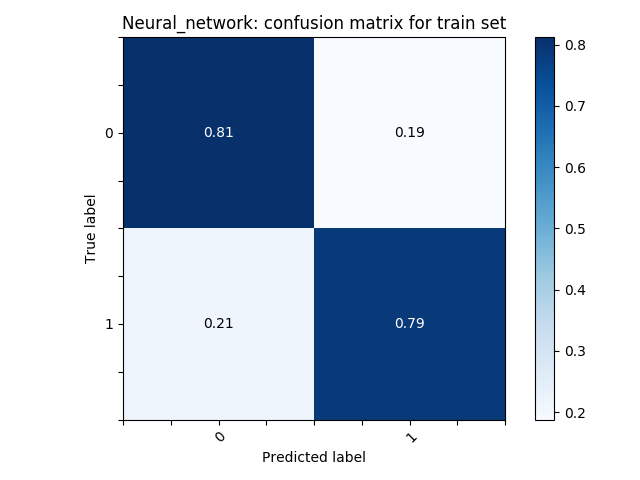
\includegraphics[width=\textwidth]{\kawFigPath /Neural_network-bank-note-cm-train.png}
        \caption{Confusion matrix of training data}\label{ligne_on}
    \end{subfigure}
    ~
    \begin{subfigure}[b]{0.45\textwidth}
        \centering 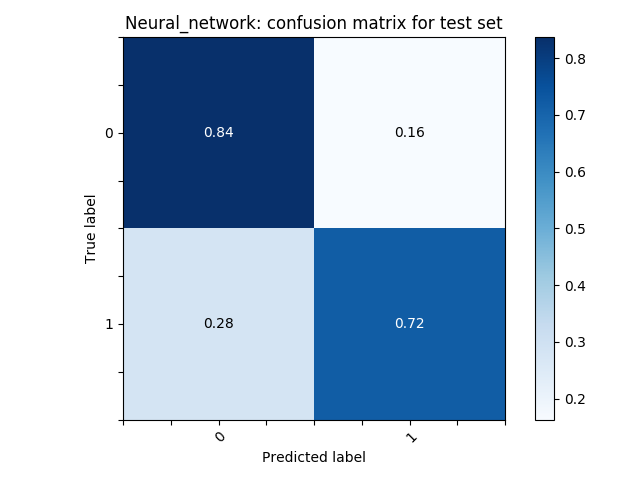
\includegraphics[width=\textwidth]{\kawFigPath /Neural_network-bank-note-cm-test.png}
        \caption{Confusion matrix test data}\label{ligne_off}
    \end{subfigure}
    \caption{Confusion matrices in the Banknote dataset}\label{figxx}
\end{figure}

\begin{figure}[H]
    \centering
    \begin{subfigure}[b]{0.45\textwidth} % "0.45" donne ici la largeur de l'image
        \centering 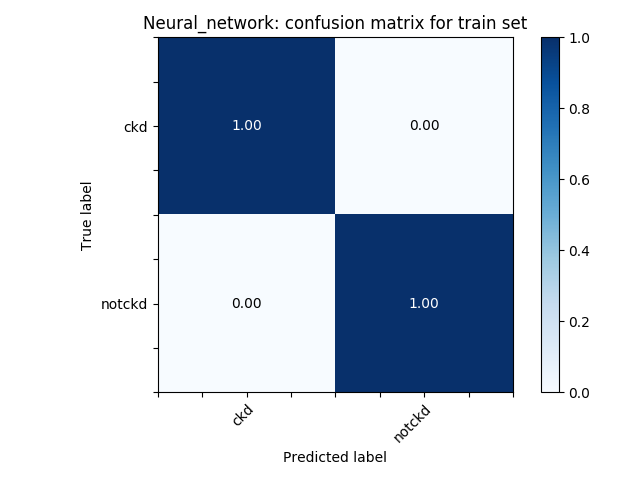
\includegraphics[width=\textwidth]{\kawFigPath /Neural_network-kidney-disease-cm-train.png}
        \caption{Confusion matrix of training data}\label{ligne_on}
    \end{subfigure}
    ~
    \begin{subfigure}[b]{0.45\textwidth}
        \centering 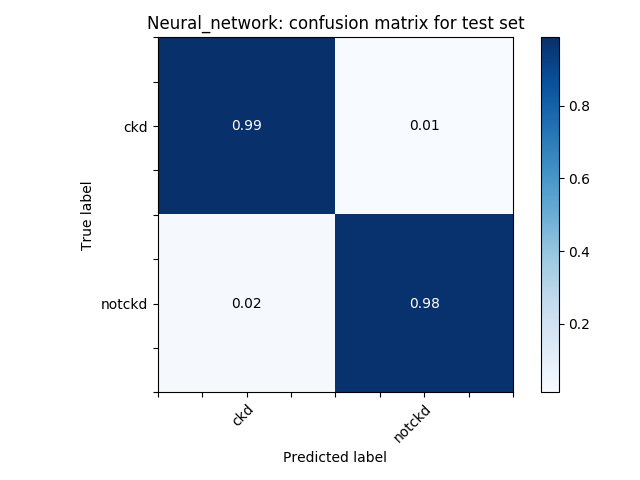
\includegraphics[width=\textwidth]{\kawFigPath /Neural_network-kidney-disease-cm-test.png}
        \caption{Confusion matrix test data}\label{ligne_off}
    \end{subfigure}
    \caption{Confusion matrices in the Kidney Disease dataset}\label{figxx}
\end{figure}

\section{Decision trees}
Decision Tree is a non-parametric supervised learning method used for both classification and regression tasks. In general, decision trees are constructed via an algorithmic method that identifies ways to split a data set based on different conditions. The decision rules are generally in form of if-then-else statements. The deeper the tree, the more complex the rules and fitter the model. In our implementation, we used skicit-learn library. The chosen splitting criteria was Gini, which favours pure nodes as it measures how often a randomly chosen element from the set would be incorrectly labeled if it was randomly labeled according to the distribution of labels in the leave. 

The following confusions matrices were obtained when running this algorithm on both datasets.It can be stated that training data are classified with no error in both datasets. For the banknote dataset, the performance of the decision tree-based classifier is perfect on the test data. Concerning the kidney disease dataset, as much as 2\% of the sick patients are diagnosed as being healthy, whereas none of the healthy patients is diagnosed as being sick. 


\begin{figure}[ht]
    \centering
    \begin{subfigure}[b]{0.45\textwidth} % "0.45" donne ici la largeur de l'image
        \centering 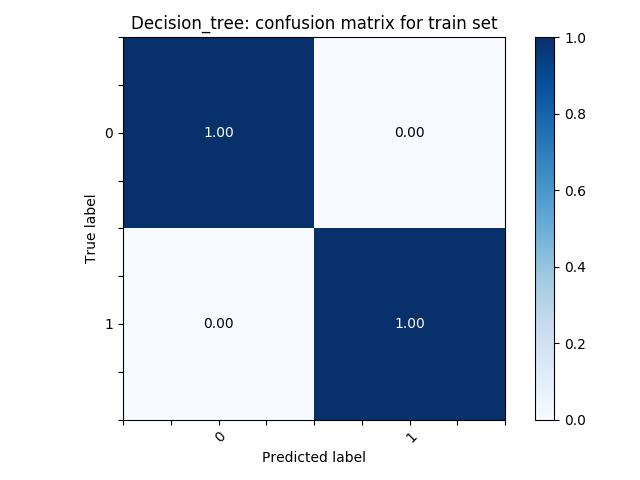
\includegraphics[width=\textwidth]{\kawFigPath /Decision_tree-bank-note-cm-train.png}
        \caption{Confusion matrix of training data}\label{ligne_on}
    \end{subfigure}
    ~
    \begin{subfigure}[b]{0.45\textwidth}
        \centering 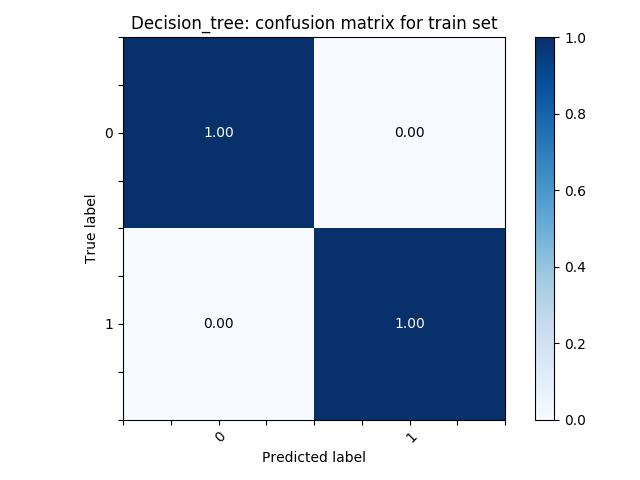
\includegraphics[width=\textwidth]{\kawFigPath /Decision_tree-bank-note-cm-train.png}
        \caption{Confusion matrix test data}\label{ligne_off}
    \end{subfigure}
    \caption{Confusion matrices in the Banknote dataset}\label{figxx}
\end{figure}
\begin{figure}[ht]
    \centering
    \begin{subfigure}[b]{0.45\textwidth} % "0.45" donne ici la largeur de l'image
        \centering 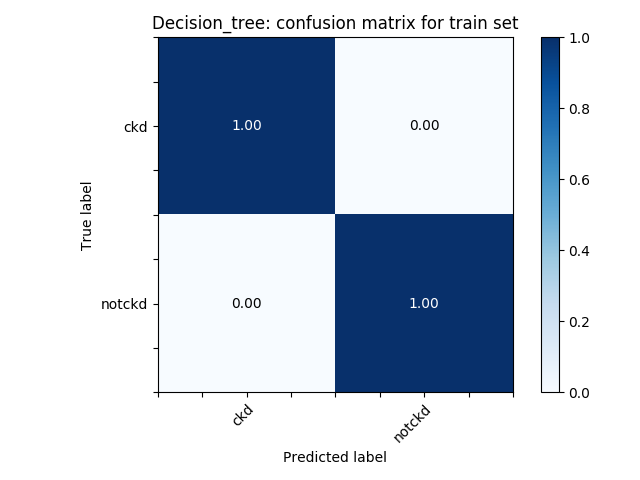
\includegraphics[width=\textwidth]{\kawFigPath /Decision_tree-kidney-disease-cm-train.png}
        \caption{Confusion matrix of training data}\label{ligne_on}
    \end{subfigure}
    ~
    \begin{subfigure}[b]{0.45\textwidth}
        \centering 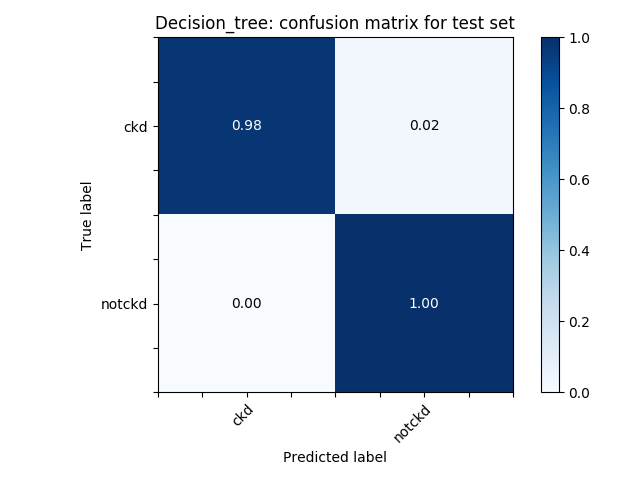
\includegraphics[width=\textwidth]{\kawFigPath /Decision_tree-kidney-disease-cm-test.png}
        \caption{Confusion matrix test data}\label{ligne_off}
    \end{subfigure}
    \caption{Confusion matrices in the Kidney Disease dataset}\label{figxx}
\end{figure}


\section{Bayesian approach}
Given a class variable $y$ and a dependent feature vector $x$, the Bayes rules states:

$$p(y|x)=\frac{p(x|y)p(y)}{p(x)}$$

Since the denominator is constant for a given input, maximizing the posterior probability $p(y|x)$ is equivalent to maximizing the numerator of the expression above. Therefore, given a feature vector $x$, its class can be estimated as it follows: 

$$\hat{y}= \arg \max\limits_{y} p(x|y)p(y)$$

$p(y)$ is estimated as the frequency of class $y$ in the dataset. The performance of the classification relies on how accurate our previous knowledge of the distribution $p(x|y)$ is. A naive yet good first approach is to model this distribution as Gaussian. 

Implementing the previous decision rule by using skicit-learn gives the confusion matrices for the considered datasets. It can be stated that the overall performance of this technique is way lower than that of the other algorithms. For example, when taking into account the Kidney Disease dataset, the test data false negative rate is as high as 7\%. This means that if we were talking about actual patients, 7\% of the sick ones would have been diagnosed as healthy. This rate is high when considering disease diagnose. 
When looking at the banknote dataset, as much as 9\% of counterfeit bills are classified as real and as much as 25\% of the real ones are classified as fake ; both indicators show the bayesian classifier is not well suited for this dataset. 


\begin{figure}[ht]
    \centering
    \begin{subfigure}[b]{0.45\textwidth} % "0.45" donne ici la largeur de l'image
        \centering 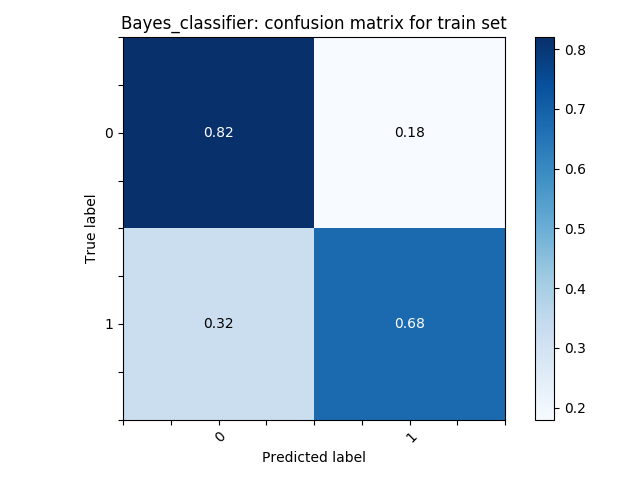
\includegraphics[width=\textwidth]{\kawFigPath /Bayes_classifier-bank-note-cm-train.png}
        \caption{Confusion matrix of training data}\label{ligne_on}
    \end{subfigure}
    ~
    \begin{subfigure}[b]{0.45\textwidth}
        \centering 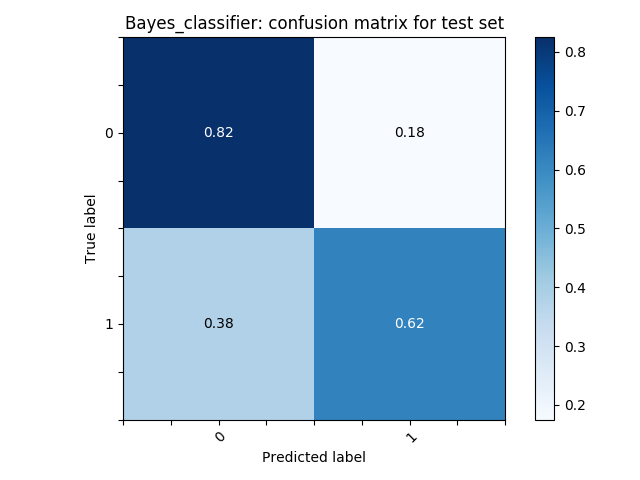
\includegraphics[width=\textwidth]{\kawFigPath /Bayes_classifier-bank-note-cm-test.png}
        \caption{Confusion matrix test data}\label{ligne_off}
    \end{subfigure}
    \caption{Confusion matrices in the Banknote dataset}\label{figxx}
\end{figure}
\begin{figure}[ht]
    \centering
    \begin{subfigure}[b]{0.45\textwidth} % "0.45" donne ici la largeur de l'image
        \centering 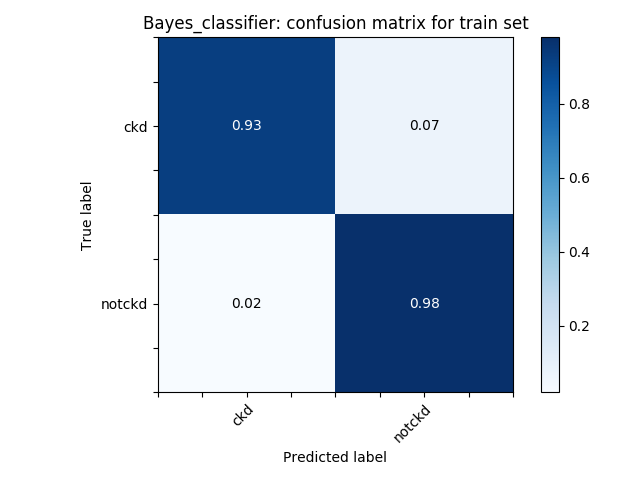
\includegraphics[width=\textwidth]{\kawFigPath /Bayes_classifier-kidney-disease-cm-train.png}
        \caption{Confusion matrix of training data}\label{ligne_on}
    \end{subfigure}
    ~
    \begin{subfigure}[b]{0.45\textwidth}
        \centering 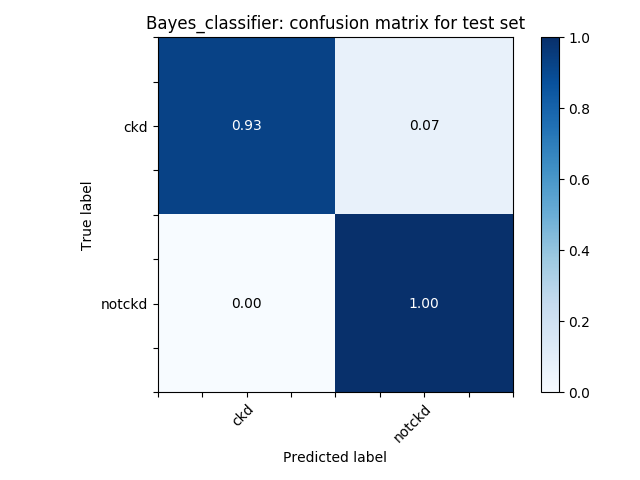
\includegraphics[width=\textwidth]{\kawFigPath /Bayes_classifier-kidney-disease-cm-test.png}
        \caption{Confusion matrix test data}\label{ligne_off}
    \end{subfigure}
    \caption{Confusion matrices in the Kidney Disease dataset}\label{figxx}
\end{figure}


This performance can be explained by errors in our modeling hypotheses. Indeed, we supposed our training data had Gaussian distribution when fixing the class $y$, which might actually be a coarse approximation. Previous statistic analysis of the data could have been performed in order to determine a better estimate of $p(x|y)$; this way, our modeling hypothesis would have fitted our training data and it would probably have led to a more acceptable performance. 

\begin{table}[ht]
\centering
\caption{Different metrics for the bank note database}
\begin{tabular}{|c|c|c|c|c|c|c|c|c|}
\hline
\rowcolor[HTML]{C0C0C0} 
\cellcolor[HTML]{C0C0C0}{\color[HTML]{333333} }                                 & \multicolumn{2}{c|}{\cellcolor[HTML]{C0C0C0}{\color[HTML]{333333} \textbf{Accuracy}}} & \multicolumn{2}{c|}{\cellcolor[HTML]{C0C0C0}{\color[HTML]{333333} \textbf{Precision}}} & \multicolumn{2}{c|}{\cellcolor[HTML]{C0C0C0}{\color[HTML]{333333} \textbf{Recall}}} & \multicolumn{2}{c|}{\cellcolor[HTML]{C0C0C0}{\color[HTML]{333333} \textbf{F1}}} \\ \cline{2-9} 
\rowcolor[HTML]{C0C0C0} 
\multirow{-2}{*}{\cellcolor[HTML]{C0C0C0}{\color[HTML]{333333} \textbf{Model}}} & \textbf{N-P}                             & \textbf{PCA}                            & \textbf{N-P}                             & \textbf{PCA}                             & \textbf{N-P}                            & \textbf{PCA}                           & \textbf{N-P}                          & \textbf{PCA}                         \\ \hline
SVM                                                                             & 1.000                                       & 0.799                                   & 1.000                                       & 0.802                                    & 1.000                                      & 0.856                                  & 1.000                                    & 0.827                                \\ \hline
KNN                                                                             & 1.000                                       & 0.843                                   & 1.000                                       & 0.844                                    & 1.000                                      & 0.887                                  & 1.000                                    & 0.865                                \\ \hline
NN                                                                              & 0.989                                       & 0.786                                   & 0.992                                       & 0.796                                    & 0.988                                      & 0.837                                  & 0.990                                    & 0.816                                \\ \hline
DT                                                                              & 0.982                                       & 0.832                                   & 0.973                                       & 0.849                                    & 0.996                                      & 0.856                                  & 0.985                                    & 0.853                                \\ \hline
BA                                                                              & 0.839                                       & 0.735                                   & 0.826                                       & 0.739                                    & 0.907                                      & 0.825                                  & 0.865                                    & 0.779                                \\ \hline
\end{tabular}
\label{tablePCA1}
\end{table}

\begin{table}[ht]
\centering
\caption{Different metrics for the kidney disease database}
\begin{tabular}{|c|c|c|c|c|c|c|c|c|}
\hline
\rowcolor[HTML]{C0C0C0} 
\cellcolor[HTML]{C0C0C0}{\color[HTML]{333333} }                                 & \multicolumn{2}{c|}{\cellcolor[HTML]{C0C0C0}{\color[HTML]{333333} \textbf{Accuracy}}} & \multicolumn{2}{c|}{\cellcolor[HTML]{C0C0C0}{\color[HTML]{333333} \textbf{Precision}}} & \multicolumn{2}{c|}{\cellcolor[HTML]{C0C0C0}{\color[HTML]{333333} \textbf{Recall}}} & \multicolumn{2}{c|}{\cellcolor[HTML]{C0C0C0}{\color[HTML]{333333} \textbf{F1}}} \\ \cline{2-9} 
\rowcolor[HTML]{C0C0C0} 
\multirow{-2}{*}{\cellcolor[HTML]{C0C0C0}{\color[HTML]{333333} \textbf{Model}}} & \textbf{N-P}                            & \textbf{PCA-2/-7}                           & \textbf{N-P}                            & \textbf{PCA-2/-7}                            & \textbf{N-P}                           & \textbf{PCA-2/-7}                          & \textbf{N-P}                         & \textbf{PCA-2/-7}                        \\ \hline
=SVM                                                                             & 0.992                                   & 1.000/1.000                                 & 1.000                                   & 1.000/1.000                                  & 0.988                                  & 1.000/1.000                                & 0.994                                & 1.000/1.000                              \\ \hline
KNN                                                                             & 0.962                                   & 0.985/0.985                                 & 1.000                                   & 1.000/1.000                                  & 0.940                                  & 0.976/0.976                                & 0.969                                & 0.987/0.987                              \\ \hline
NN                                                                              & 0.985                                   & 0.985/0.992                                 & 0.988                                   & 1.000/1.000                                  & 0.988                                  & 0.976/0.988                                & 0.988                                & 0.987/0.994                              \\ \hline
DT                                                                              & 0.985                                   & 0.985/0.977                                 & 1.000                                   & 0.976/1.000                                  & 0.976                                  & 1.000/0.964                                & 0.988                                & 0.988/0.981                              \\ \hline
BA                                                                              & 0.955                                   & 0.924/0.924                                 & 1.000                                   & 0.986/0.974                                  & 0.928                                  & 0.893/0.905                                & 0.963                                & 0.938/0.938                              \\ \hline
\end{tabular}
\label{tablePCA2}
\end{table}

\section{Discussion on good programming practices}
Through this work, we realized organized coding is an important skill in machine learning and it is as important as having good bases on statistics and mathematics. This allows anyone who reads the developed codes understanding what has been done and it also facilitates further modifications if they are necessary.

Comments are important for understanding the code, and this even applies to the code's authors so they can remember what the code is about if they ever stop using it for a while. Naming conventions for variables, functions and variables are also important for the code's understanding; if adequate names are used, codes understanding becomes easier and more intuitive. Our codes were implemented by using the conventions most currently used in machine learning: $x$ for the features, $y$ for the classes, etc. By doing this, the need for comments or documentation can significantly be reduced, since the names themselves are representative enough for someone familiarized with machine learning. 

We structured our project's repository as it follows: first, we created a main executable file that includes everything we need to run in this project. We did our best to develop this file by including a low quantity of logical functions that allow understanding the dependency relationships between different blocks in the repository.  We also created a utilities file that includes functions that were  called by our different models and that assured different useful functionalities. Finally, we created an independent module for data pre-processing as well as a module where the different models (machine learning algorithms) were loaded.

A readme file was also generated so somebody who didn't develop the repository could easily understand it. Documenting our code makes it more user friendly and facilitates collaborative work. We also used version control; this functionality allows to keep a record of what's been done in the project; it allows going back at a certain point if some undesired modifications are made and it facilitates assembling different parts of a code when different people work in parallel. 

\section*{Conclusion}
The performance of all considered algorithms in terms of different metrics is presented in tables \ref{tablePCA1} and \ref{tablePCA2} (\textbf{N-P}\footnote{Results of the algorithms without using PCA}).
Through this document, we exposed the implementation of different machine learning algorithms on two different datasets. The analysis of their performance relies on the metric we use, and the choice of the metric isn't evident since it depends on the nature of the problem itself. For example, when studying the Kidney Disease dataset some of the algorithms threw a false negative rate of about 2\%. However, if the test is applied on a population that happens to have a million sick people, this apparently small percentage would mean two thousand people who do have the disease would be incorrectly diagnosed, which wouldn't be acceptable. 

Different algorithms were tested and every single one of them needs an appropriate tuning of different parameters which may heavily influence the classification result : the kernel in SVM, the number of neighbors considered in KNN, the architecture of the neural network and the choice of the activation functions, the depth of decision trees and the stop criteria, the prior probability density in bayesian approach. None of those choices is evident, and a slight change in some of them may lead to significantly different results. We adapted different parameters in order to get what we consider is an acceptable performance for each classifier, but that doesn't mean the performance of every single one of them can't be improved. 

Performance was established on the base of test data corresponding to 1/3 of the dataset (training data corresponded to 2/3 of the dataset). A cross-validation technique would have allowed us verifying if the performances we determined do correspond to a tendency. 

The project gave us a better and more practical understanding of the different algorithms we treated during machine learning and, last but not least, it constituted a valuable experience for us since it encouraged collaborative team-work as well as good programming practices we'll surely need in a close future.  

\section*{References}
Guyon, I., Boser, B. and Vapnik, V. (1993). Automatic Capacity Tuning of Very Large VC-dimension Classifiers. Advances in Neural Information Processing Systems.

Goldberger, J., Roweis, S., Hinton, G. and Salakhutdinov, R. (1993). Neighbourhood Components Analysis.

Quinlan, J.R. (1993). C4. 5: programs for machine learning. Morgan Kaufmann.

Zhang, H. (2005). Exploring conditions for the optimality of naïve bayes. International Journal of Pattern Recognition and Artificial Intelligence, 19(02), pp.183-198.

\newpage
\appendix
\section{The logs of your git}
\begin{verbatimprog}

* 71ef4df - (hace 4 horas) PCA some modification: panda dataframe, only take in
                the second database the numerical ones and concatenate with the categorical
    ones - sagudelor (HEAD -> master, origin/master, origin/HEAD)
* 6bf17b9 - (hace 21 horas) Report v0.2.1 - sagudelor
* 44faa22 - (hace 21 horas) Report v0.2 - sagudelor
* d2646a3 - (hace 22 horas) Modification name of some models - sagudelor
* 67172f0 - (hace 26 horas) Update README.md - Tales Marra
* 53bd23b - (hace 29 horas) adding pca - talesmarra
*   2afb4fe - (hace 30 horas) mod - talesmarra
|\  
| * 7dc3e8d - (hace 2 días) Report v0.1 - sagudelor
| * ddd63a3 - (hace 2 días) Update README.md - Tales Marra
| * 7586624 - (hace 2 días) Update README.md - Tales Marra
| * fbb969c - (hace 2 días) verbose set to off, accuracy precision set to three decimals - gonzaq94
| * 67f12fa - (hace 2 días) some comments made, unnecessary import deleted - gonzaq94
| * 3e5d566 - (hace 2 días) image and file naming problem resolved - gonzaq94
| *   38f0e83 - (hace 2 días) Merge branch 'master' of https://github.com/talesmarra/UE_ML_project - gonzaq94
| |\  
| | * 9a61d58 - (hace 2 días) Delete requirements.txt - Gonzalo Quintana
| * | 741f41d - (hace 2 días) export file created and change in filename - gonzaq94
| * | 0d2d3af - (hace 2 días) export file created and change in filename - gonzaq94
| * | 71c4047 - (hace 2 días) export file created and change in filename - gonzaq94
| * | 3f65807 - (hace 2 días) export file created and change in filename - gonzaq94
| * | 42841fb - (hace 2 días) export file created and change in filename - gonzaq94
* | | dda523a - (hace 31 horas) Images - talesmarra
| |/  
|/|   
* | 0514ee1 - (hace 2 días) adding reqs - talesmarra
* | 1d86ba6 - (hace 2 días) fixing nn - talesmarra
|/  
*   bc2298a - (hace 2 días) Merge branch 'master' of https://github.com/talesmarra/UE_ML_project - talesmarra
|\  
| * 2695154 - (hace 2 días) Some changes - sagudelor
* | 864fa4b - (hace 2 días) fixing knn - talesmarra
* | 3d08a4d - (hace 2 días) fixing knn - talesmarra
|/  
* 4029b13 - (hace 9 días) fixing logo - Tales Marra
* 3831a54 - (hace 9 días) Update README.md - Tales Marra
* a40dc73 - (hace 9 días) adding parser and bayes - talesmarra
* b13c3fd - (hace 3 semanas) Delete tp-svms-quintana-marra.ipynb - Tales Marra
*   4b80298 - (hace 3 semanas) comments - talesmarra
|\  
| * d73c0cf - (hace 3 semanas) confusion matrix images correctly showed and saved - gonzaq94
| * 9933ca1 - (hace 3 semanas) small change in main function - gonzaq94
| * 1ff328c - (hace 3 semanas) merge finished - gonzaq94
| * 5c78d23 - (hace 3 semanas) labels added to confusion matrix - gonzaq94
| *   57d5412 - (hace 3 semanas) small merge - gonzaq94
| |\  
| | * 4b328c0 - (hace 3 semanas) Labels of the target in the binarization option - sagudelor
| * | a545092 - (hace 3 semanas) small changes in main - gonzaq94
| |/  
| * 4c957af - (hace 3 semanas) merge between data preprocessing and main progra 
|            successfully done - Gonzalo QUINTANA
| * 2ff8359 - (hace 3 semanas) Cleaning and scale data - sagudelor
| *   0692371 - (hace 3 semanas) Cleaning data and scale - sagudelor
| |\  
| | * e03d52d - (hace 3 semanas) data import and string detection - wang-lei-cn
| * | b23f7db - (hace 3 semanas) Data cleaning and scale - sagudelor
| |/  
| * 714bc56 - (hace 3 semanas) Data for the classifictation - sagudelor
| * 75fddda - (hace 3 semanas) main function with training and testing completed - Gonzalo QUINTANA
* | f7e51a1 - (hace 3 semanas) change kmeans - talesmarra
|/  
* 68c1d26 - (hace 3 semanas) change nn - talesmarra
* a270c5f - (hace 3 semanas) fixing neural network - talesmarra
* c5d50a8 - (hace 3 semanas) models - talesmarra
* 4c22cfb - (hace 4 semanas) tp for database - talesmarra
* 0f03b2b - (hace 4 semanas) Initial commit - Tales Marra

\end{verbatimprog}

\section{Code of the project}
\subsection{main.py}
\begin{lstlisting}[language=Python,basicstyle=\tiny]
from models import *
from utilities import *
from prepro import *
import argparse
import sys

if __name__ == "__main__":

    # Some general parameters

    output_folder = "Output"
    accs_file_path = output_folder + "/accuracies_file"
    test_size = 0.33

    # Dataset and models to use are passed by command

    parser = argparse.ArgumentParser()
    parser.add_argument('--models', type=str, help='the list of models you want to use',
                        default='svm_model')

    parser.add_argument('--dataset', type=str, default='kidney-disease',
                        help='Dataset to use: either kidney-disease or '
                             'bank-note ')
    parser.add_argument('--do_pca', help='If you want ot perform PCA', action='store_true')
    args = parser.parse_args()

    models_string = [item for item in args.models.split(',')]
    if args.dataset == 'kidney-disease':
        path = "data_classification/kidney_disease.csv"
        accs_file_path = accs_file_path + '_kidney_disease.txt'
        X, y, label, mod = load_preprocessing_data(path, index_col=0, binar=True)  # for kidney_disease
    elif args.dataset == 'bank-note':
        path = "data_classification/data_banknote_authentication.txt"
        accs_file_path = accs_file_path + '_bank_note.txt'
        X, y, label, mod = load_preprocessing_data(path, header=None, binar=True)  # for banknote
    else:
        print('dataset not available or misspelled')
        sys.exit(1)

    y_labels = [label[0], label[1]]
    if args.do_pca:
        DO_PCA = True
        if args.dataset == 'kidney-disease':
            X = pca(X, 'kidney-disease', mod)
        else:
            X = pca(X, 'bank-note', mod)
    else:
        DO_PCA = False

    # load preprocessed data

    X_train, X_test, y_train, y_test = data_split(X, y, test_size)
    if args.dataset == 'kidney-disease':
        models = call_models(models_string, 'kidney-disease', DO_PCA)
    else:
        models = call_models(models_string, 'bank-note', DO_PCA)

    # create the output files

    if not os.path.exists(output_folder):
        os.makedirs(output_folder)
        os.makedirs(output_folder + '/Images')

    accs_file = create_accs_file(accs_file_path, args.dataset)

    for i, model in enumerate(models):
        train_model(model, X_train, np.ravel(y_train))

        accuracy = validation(model, X_test, y_test)

        print(models_string[i], ' accuracy: ', '%.3f' % accuracy)

        print_acc_2_file(accs_file, models_string[i], accuracy)

        # we plot the confusion matrix for both the train and test datasets

        plot_confusion_matrix(model, X_train, y_train, models_string_dic[models_string[i]], y_labels, train_flag=True,
                              dataset=args.dataset)

        plot_confusion_matrix(model, X_test, y_test, models_string_dic[models_string[i]], y_labels, train_flag=False,
                              dataset=args.dataset)
\end{lstlisting}

\subsection{models.py}
\begin{lstlisting}[language=Python,basicstyle=\tiny]
import keras
import sklearn
from keras.layers import Dense
from sklearn import tree, svm
from sklearn.neighbors import KNeighborsClassifier
from sklearn.naive_bayes import GaussianNB


def svm_model():
    """
    :return: instance of the model
    """
    return svm.SVC(gamma='scale')


def knn_model():
    """
    :return: instance of the model
    """
    return KNeighborsClassifier(n_neighbors=5)


def decision_tree_model():
    """
    :return: instance of the model
    """
    return tree.DecisionTreeClassifier()


def neural_network(input_dim, n_neurons_per_layer=None, n_layers=3):
    """
    :return: instance of the model
    """
    if n_neurons_per_layer is None:
        n_neurons_per_layer = [5, 3, 2]
    if len(n_neurons_per_layer) != n_layers:
        print('number of layers of network not match number of neurons per layer')
    else:
        classifier = keras.Sequential()
        # Input layer
        classifier.add(
            Dense(n_neurons_per_layer[0], activation='relu', kernel_initializer='random_normal',
                  input_dim=input_dim))
        for n in n_neurons_per_layer[1:]:
            # Hidden Layers
            classifier.add(Dense(n, activation='tanh', kernel_initializer='random_normal'))

            # Output Layer
        classifier.add(Dense(1, activation='sigmoid', kernel_initializer='random_normal'))

        # Compiling the neural network
        classifier.compile(optimizer='adam', loss='binary_crossentropy', metrics=['accuracy'])
        return classifier


def gaussian_bayes_model():
    """

    :return:Gaussian Naive Bayes (GaussianNB)
    """
    return GaussianNB()


def call_models(list_models, dataset, do_pca):
    """
    :param do_pca: if to do pca or not
    :param dataset: type of dataset
    :param: list_models: the names of the models you want to use
    :type list_models: list
    """
    list_of_models = list()
    for model in list_models:
        if type(model) == str:
            if model == 'svm_model':
                list_of_models.append(svm_model())
            elif model == 'knn_model':
                list_of_models.append(knn_model())
            elif model == 'decision_tree_model':
                list_of_models.append(decision_tree_model())
            elif model == 'bayes_model':
                list_of_models.append(gaussian_bayes_model())
            elif model == 'neural_network':
                if dataset == 'kidney-disease':
                    if do_pca:
                        input_dim = 10
                    else:
                        input_dim = 24
                else:
                    if do_pca:
                        input_dim = 2
                    else:
                        input_dim = 4
                try:
                    list_of_models.append(neural_network(input_dim))
                except:
                    print('Not loaded neural network')
                    continue
    return list_of_models

\end{lstlisting}

\subsection{prepro.py}
\begin{lstlisting}[language=Python,basicstyle=\tiny]
# Copyright (c) 2019, IMT Atlantique
# All rights reserved.

# ==============================================================================
"""Contains differents functions for the preprocessing of the data."""
import re
import pandas as pd
import os
import numpy as np
from sklearn import preprocessing
from sklearn.decomposition import PCA
from mlxtend.plotting import plot_pca_correlation_graph
import matplotlib.pyplot as plt


def load_preprocessing_data(path, header='infer', index_col=None, binar=False):
    df = pd.read_csv(path, header=header, index_col=index_col)
    lines = df.shape[0]
    columns = df.shape[1]
    x = df.drop(df.columns[columns - 1], axis=1)
    y = df.take([-1], axis=1)

    varx, xn = stringDetection(x)
    print("String detection process done")
    vary, yn = stringDetection(y)
    print("String detection process done")

    # cleaning

    vary, yn, mody, labely = cleaning(vary, yn, binar, target=True)
    varx, xn, modx, labelx = cleaning(varx, xn, binar, target=False)

    # validation
    if yn.isnull().any().all():
        print("Error in the cleaning process")
    else:
        print("Cleaning process done")
    if yn.isnull().any().all():
        print("Error in the cleaning process")
    else:
        print("Cleaning process done")

    # scale and normalize
    xn = scale_norm(xn, varx, modx)
    print("Scaling and normalize process done")
    print(labely)
    return xn, yn, labely, modx


def scale_norm(xn, var, mod):
    for i in range(len(var)):
        if mod[i] == 'numeric':
            xn.loc[:, xn.columns[i]] = pd.DataFrame(preprocessing.scale(xn[xn.columns[i]]), columns=[xn.columns[i]])
    return xn


def stringDetection(x):
    """
    x as a pandas array
    """
    xn = pd.DataFrame(columns=x.columns, index=x.index)
    var = []

    for j in range(x.shape[1]):
        j = []
        var.append(j)
    for i, row in enumerate(x.values):
        for j in range(x.shape[1]):
            try:
                row[j] = float(row[j])
            except ValueError:
                row[j] = row[j]
            if isinstance(row[j], str):
                row[j] = re.sub(r"[^a-zA-Z0-9]+", '', row[j])
                if ((row[j] in var[j]) == False) and (row[j] != ''):
                    var[j].append(row[j])
                if (row[j] == ''):
                    row[j] = float('nan')
        xn.loc[i] = row

    return var, xn


def replacement(xn, mod):
    xf = pd.DataFrame(np.zeros(shape=(xn.shape[0], 1)), columns=[xn.name], index=np.arange(0, xn.shape[0]))
    if mod == 2:
        p = xn.mean()
        m = xn.isnull().sum()
        v = np.random.binomial(1, round(p, 2), m)
        j = 0
        for k in range(xn.shape[0]):
            if np.isnan(xn[k]):
                xf.loc[k] = v[j]
                j += 1
            else:
                xf.loc[k] = xn[k]
    return xf


def cleaning(var, xn, binar, target):
    mod = []
    label = {}
    for i in range(len(var)):

        if not var[i]:

            mod.append('numeric')
            xn[xn.columns[i]].fillna(float(xn[xn.columns[i]].mean()), inplace=True)
        else:
            mod.append('modal')
            if binar:
                Ncases = len(var[i])
                v = [i for i in range(len(var[i]))]
                # print("Binarization...", xn.columns[i])
                xn[xn.columns[i]] = xn[xn.columns[i]].replace(var[i], v)
                if target:
                    for k in range(len(v)):
                        label[v[k]] = var[i][k]
                var[i] = []

                # print(xn[xn.columns[i]].mean())

                xn.loc[:, xn.columns[i]] = replacement(xn[xn.columns[i]], Ncases)
                # print(xn[xn.columns[i]].mean())
            else:
                xn[xn.columns[i]].fillna(method='bfill', inplace=True)
    if not label and target:
        labels = list(set(xn[xn.columns[0]]))
        v = [i for i in range(len(labels))]
        for k in range(len(v)):
            label[v[k]] = labels[k]

    return var, xn, mod, label


def pca(x, dataset, mod):
    """

    :param x:
    :param dataset:
    :return:
    """
    xn = x[list(x.columns[np.argwhere(np.array(mod)=='numeric')])]
    xm = x[list(x.columns[np.argwhere(np.array(mod)=='modal')])]
    if dataset == 'kidney-disease':
        n = 10
        pca_instance = PCA(n_components=n)
        pca_instance.fit(xn[list(xn.columns)])
        xp = pca_instance.transform(xn)
        var = sum(pca_instance.explained_variance_[:n]) * 100 / sum(pca_instance.explained_variance_)
        print('The {} principal components are responsible for {}% of the variance'.format(n, var))
        feature_names = list(xn.columns)
        figure, correlation_matrix = plot_pca_correlation_graph(xn, feature_names, figure_axis_size=10)
        plt.savefig('Output/Images' + "/" + 'PCA_for_dataset_{}'.format(dataset))
        plt.close()
        xp = pd.DataFrame(data = xp, index=xn.index)
        xp = pd.concat([xp, xm], axis=1)
        return xp
    elif dataset == 'bank-note':
        n = 2
        pca_instance = PCA(n_components=n)
        pca_instance.fit(x)
        xp = pca_instance.transform(x)
        var = sum(pca_instance.explained_variance_[:n]) * 100 / sum(pca_instance.explained_variance_)
        print('The {} principal components are responsible for {}% of the variance'.format(n, var))
        feature_names = ['variance', 'skewness', 'curtosis', 'entropy']
        figure, correlation_matrix = plot_pca_correlation_graph(x, feature_names, figure_axis_size=10)
        plt.savefig('Output/Images' + "/" + 'PCA_for_dataset_{}'.format(dataset))
        plt.close()
        return xp

\end{lstlisting}

\subsection{utilities.py}
\begin{lstlisting}[language=Python,basicstyle=\tiny]
from sklearn.model_selection import train_test_split
from sklearn.metrics import confusion_matrix, accuracy_score
from keras import Sequential
import matplotlib.pyplot as plt
import numpy as np


def data_split(X, y, test_size):
    """

    :param X: input data
    :param y: input labels
    :param test_size: percentage of dataset used for test
    :return: the splitted data
    """

    X_train, X_test, y_train, y_test = train_test_split(X, y, test_size=test_size, random_state=42)

    return X_train, X_test, y_train, y_test


def train_model(model, x, y, epochs=50):
    """

    :param model: the model that will be used for training
    :param x: input data
    :param y: input labels
    :param epochs: number of epochs for training
    :return: the trained model
    """
    if isinstance(model, Sequential):

        model.fit(x, y, epochs=epochs, verbose=0)

    else:
        model.fit(x, y)

    return model


def validation(model, x, y):
    """

    :param model: instance of a model
    :param x: input data
    :param y: input labels
    :return: the accuracy score obtained
    """
    if isinstance(model, Sequential):

        y_pred = model.predict(x)

        y_pred = np.array([y_pred > 0.5]).astype(np.int16)

        y_pred = y_pred.reshape(len(y))

        return accuracy_score(y, y_pred)

    else:

        return model.score(x, y)


def plot_confusion_matrix(model, x, y_true, model_string, cm_labels, train_flag, dataset, image_folders="Output/Images"):
    """

    :param model: instance of the model
    :param x: input data
    :param y_true: true labels
    :param model_string: name of model
    :param cm_labels: type of colormap
    :param train_flag: true if train, else false
    :param dataset: dataset used,for naming the image
    :param image_folders: folder to save images
    :return:
    """
    y_pred = model.predict(x)

    if isinstance(model, Sequential):
        y_pred = np.array([y_pred >= 0.5]).astype(np.int)

        y_pred = y_pred.reshape(len(y_true))

    cm = confusion_matrix(y_true, y_pred)

    # we normalize the confusion matrix
    print(cm)
    cm = cm.astype('float') / cm.sum(axis=1)[:, np.newaxis]

    fig, ax = plt.subplots()

    # we plot

    im = ax.imshow(cm, interpolation='nearest', cmap=plt.cm.Blues)
    ax.figure.colorbar(im, ax=ax)

    fmt = '.2f'
    thresh = cm.max() / 2
    for i in range(cm.shape[0]):
        for j in range(cm.shape[1]):
            ax.text(j, i, format(cm[i, j], fmt),
                    ha="center", va="center",
                    color="white" if cm[i, j] > thresh else "black")

    if train_flag:
        title = model_string + ": confusion matrix for train set"
        fig_name = model_string + '-' + dataset + '-cm-train.png'
    else:
        title = model_string + ": confusion matrix for test set"
        fig_name = model_string + '-' + dataset + '-cm-test.png'

    labels = ['', '', cm_labels[0], '', '', '', cm_labels[1]]

    ax.set(  # xticks=np.arange(cm.shape[1]),
        # yticks=np.arange(cm.shape[0]),
        # ... and label them with the respective list entries
        xticklabels=labels, yticklabels=labels,
        title=title,
        ylabel='True label',
        xlabel='Predicted label')

    # Rotate the tick labels and set their alignment.
    plt.setp(ax.get_xticklabels(), rotation=45, ha="right",
             rotation_mode="anchor")

    fig.tight_layout()

    plt.savefig(image_folders + "/" + fig_name)
    plt.close()

def create_accs_file(filepath, dataset):
    """

    :param filepath: accuracy file location
    :param dataset: dataset name
    :return: file
    """

    accs_file = open(filepath, "w+")

    accs_file.write("Accuracy file for: " + dataset + " dataset" + "\n")

    return accs_file


def print_acc_2_file(file, model, accuracy):
    """

    :param file: file where to write
    :param model: model name
    :param accuracy: accuracy obtained with that model
    :return:
    """

    acc_str = '%.3f' % accuracy

    file.write(models_string_dic[model] + ": " + acc_str +"\n")


# Dictionary used to set the image title more properly

models_string_dic = {
    'decision_tree_model': 'Decision_tree',
    'knn_model': 'KNN',
    'svm_model': 'SVM',
    'neural_network': 'Neural_network',
    'bayes_model': 'Bayes_classifier'
}
\end{lstlisting}



\end{document}